\documentclass[../calc1-main.tex]{subfiles}

\begin{document}

  \begin{table}[H]
    \centering
    \begin{tabular}{c|c}
      $f(x)$ & $f'(x)$ \\
      \hline
      & \\
      $x^3/3$ & $x^2$ \\
      $x^2/2$ & $x$ \\
      $x$ & $1$ \\
      $x^0$ & $0$ \\
      $-x^{-1}$ & $x^{-2}$ \\
      $-x^{-2}/2$ & $x^{-3}$
    \end{tabular}
    \caption{What is the mysterious function whose derivative is $x^{-1}$?}
  \end{table}

  \begin{definition}
    For $x>0$, let $A_x$ be the area bounded by the curve $y = 1/t$, the t-axis and the vertical lines $t=1$ and $t=x$. The \textbf{natural logarithm} function is defined by
    \[
      \ln x =
      \begin{cases}
        A_x & x \geq 1 \\
        -A_x & 0 < x < 1
      \end{cases}
    \]
  \end{definition}
  \begin{figure}[H]
    \centering
    \begin{tikzpicture}
  \begin{axis}[
  xmin=0, xmax= 3, ymin=0, ymax=6,
  xlabel=$t$, ylabel=$y$,
  xtick={1, 2},
  xticklabels={1, $x$},
  yticklabels={,,},
  axis lines=left]
  \addplot[blue, domain=.2:3, samples=100]  {1/x} node[above left]{$y=1/t$};
  \draw[dashed] (1,0) -- (1,1);
  \draw[dashed] (2,0) -- (2,.5);
  \addplot+[mark=none,
          domain=1:2,
          samples=100,
          pattern=north west lines,
          draw=blue,
          pattern color=blue,
          area legend] {1/x} \closedcycle;
\end{axis}
\end{tikzpicture}
  \end{figure}


  \begin{multicols}{2}
    \begin{itemize}
      \item Domain of $\ln x$ is $(0, \infty)$,
      \item $\ln 1 = 0$,
      \item $\ln x >0$ if $x>1$,
      \item $\ln x < 0$ if $0<x<1$,
    \end{itemize}
  \end{multicols}

  \begin{theorem}
    If $x>0$ then $\dfrac{d}{dx} \ln x = \dfrac{1}{x}$
  \end{theorem}

  \begin{proof}
    \begin{minipage}{0.4\textwidth}
      For $h >0$, $\ln(x+h) - \ln x$ is the area under $1/t$ between $t = x$ and $t = x+h$. Thus
      \[
        \frac{h}{x+h} < \ln(x+h) - \ln x < \frac{h}{x}
      \]

      Thus
      \[
        \frac{1}{x+h} < \frac{\ln(x+h) - \ln x}{h} < \frac{1}{x}
      \]
      Now use Squeeze Theorem to get
      \[
        \lim_{h \to 0+} \frac{\ln(x+h) - \ln x}{h} = \frac{1}{x}
      \]
      Similar argument holds for $h<0$.
    \end{minipage}%
    \begin{minipage}{0.6\textwidth}
      \begin{figure}[H]
        \centering
        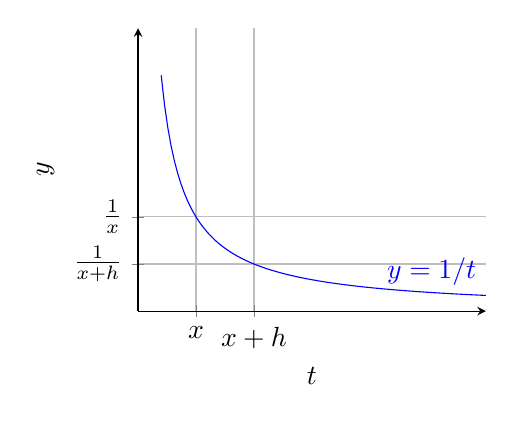
\begin{tikzpicture}
  \begin{axis}[
  width=6cm,
  grid=major,
  xmin=0, xmax= 3, ymin=0, ymax=6,
  xlabel=$t$, ylabel=$y$,
  xtick={.5, 1},
  xticklabels={$x$, $x+h$},
  ytick={1, 2},
  yticklabels={$\frac{1}{x+h}$,$\frac{1}{x}$},
  axis lines=left]
  \addplot[blue, domain=.2:3, samples=100]  {1/x} node[above left]{$y=1/t$};
\end{axis}
\end{tikzpicture}
      \end{figure}
    \end{minipage}
  \end{proof}

  \begin{theorem}
    If $x \neq 0$ then
    \[
      \frac{d}{dx} \ln \abs{x} = \frac{1}{x},
    \]
    and
    \[
      \int \frac{1}{x} dx = \ln \abs{x} + C.
    \]
  \end{theorem}
  \begin{proof}
    If $x<0$, then by Chain Rule,
    \[
      \frac{d}{dx} \ln\abs{x} = \frac{d}{dx} \ln (-x) = \frac{1}{-x} (-1) = \frac{1}{x}.
    \]
  \end{proof}

  This also shows that $\ln x$ is an \textbf{increasing} function for all $x>0$.
  \begin{example}
    Find the derivatives of
    \begin{enumerate}
      \item $y = \ln \abs{\cos x}$
      \item $y = \ln(x + \sqrt{x^2+1})$
    \end{enumerate}
  \end{example}

  \begin{solution}
    For (1),
    \[
      y' = \frac{1}{\cos x} (-\sin x) = -\tan x.
    \]
    For (2),
    \[
      y' = \frac{1}{\sqrt{x^2 + 1}}.
    \]
  \end{solution}

  The natural logarithm function $\ln x$ satisfies all the rules that the regular logarithms satisfy, that's why we call it natural log after all!
  \begin{theorem}
    \begin{enumerate}
      \item $\ln (xy) = \ln x + \ln y$.
      \item $\ln (1/x) = -\ln x$.
      \item $\ln (x/y) = \ln x - \ln y$.
      \item $\ln x^r = r \ln x$.
    \end{enumerate}
  \end{theorem}

  \begin{proof}
    For (i), if $y$ is constant, then for all $x>0$
    \[
      \frac{d}{dx} (\ln(xy)-\ln x) = \frac{y}{xy} - \frac{1}{x} = 0
    \]
    Thus for each $y>0$, $\ln(xy)-\ln x=C$ (a constant depending on $y$) for $x>0$. Setting $x=1$ we get $C=\ln y$. The others can be done similarly (homework).
  \end{proof}


  Also note that
  \[
    \ln 2^n = n \ln 2 \to \infty \text{ as } n\to \infty.
  \]
  \[
    \ln 2^{-n} = -n \ln 2 \to -\infty \text{ as } n\to \infty.
  \]
  This, combined with $\ln x$ is increasing shows that
  \[
    \lim_{x \to \infty} \ln x = \infty, \qquad
    \lim_{x \to 0+} \ln x = -\infty.
  \]

  Thus domain of $\ln x$ is $(0, \infty)$ and the range of $\ln x$ is $(-\infty, \infty)$.

  \subsection*{The Exponential Function}

  Let $f(x) = \ln x$. Since $f'(x) = 1/x > 0$ $\implies$ $f$ is increasing $\implies$ $f$ is 1-1 $\implies$ $f$ has an inverse. Call its inverse $\exp x$. Thus
  \[
    \exp x = y \iff x = \ln y
  \]

  \begin{itemize}
    \item $\exp 0 = 1$ (since $\ln 1 = 0$),
    \item Domain of $\exp$ is $(-\infty, \infty)$ (since range of $\ln$ is $(-\infty, \infty)$),
    \item Range of $\exp$ = Domain of $\ln$ = $(0, \infty)$,
    \item Cancellation identities
    \begin{align*}
      & \exp \ln x = x, \quad x>0 \\
      & \ln \exp x = x, \quad -\infty<x<\infty.
    \end{align*}
  \end{itemize}

  \begin{definition}
    $e = \exp(1) \approx 2.718 \dots$.
  \end{definition}
  Thus $\ln e = 1$. Hence $e$ is the number for which the area bounded by $y=1/x$, the x-axis and the lines $x=1$, $x=e$ is 1.

  \[
    e^x = \exp(\ln(e^x)) = \exp(x \ln e) = \exp(x).
  \]

  % \textit{To be rigorous, this holds when $x$ is rational. When $x$ is irrational we use $\exp x$ to define $e^x$.}

  Since $\exp$ is actually an exponential function, its inverse must be a logarithm
  \[
    \ln x = \log_e x
  \]

  The derivative of $y = e^x$ is calculated by implicit differentiation:
  \[
    y = e^x \iff
    x = \ln y \iff
    1 = \frac{y'}{y} \iff
    y' = y = e^x
  \]
  This is a remarkable property:
  \[
    \frac{d}{dx} e^x = e^x, \qquad \int e^x dx = e^x + C
  \]

  \begin{example}
    Find the derivatives of
    \begin{enumerate}
      \item $e^{x^2-3x}$,
      \item $\sqrt{1+e^{2x}}$
    \end{enumerate}
  \end{example}

  \subsection*{General Exponentials and Logaritms}
  \begin{definition}
    If $a>0$ then for all real $x$, we define
    \[
      a^x = e^{x \ln a}
    \]
  \end{definition}
  This coincides with our previous definition that $a^x$ is the limit of $a^{r_n}$ where $r_n$ are rational numbers tending to $x$.

  \begin{example}
    $2^{\pi} = e^{\pi \ln 2} \approx 8.825$.
  \end{example}

  \textbf{Derivative of $y=a^x$.}
  \[
    \frac{d}{dx} a^x = \frac{d}{dx} e^{x \ln a} = e^{x \ln a} \ln a = a^x \ln a.
  \]

  \begin{example}
    Show that the graph of $f(x) = x^{\pi} - \pi^x$ has negative slope at $x = \pi$.
  \end{example}
  \begin{solution}
    $f'(\pi) = \pi^{\pi} (1- \ln \pi)$. Note that $\ln \pi > \ln e = 1$
  \end{solution}

  \begin{definition}
    Let $y = a^x$. Then $\frac{dy}{dx} = a^x \ln a$ which is negative if $0<a<1$ and positive if $a>1$. Thus $a^x$ is 1-1 and has an inverse function. We define its inverse as $\log_a x$.
  \end{definition}
  \textbf{Derivative of $y=\log_a x$.}
  \[
    \frac{d}{dx} \log_a x = \frac{d}{dx} \frac{\ln x}{\ln a} = \frac{1}{a x}.
  \]

  \subsection*{Logarithmic Differentiation}

  \begin{example}
    Let $y = x^x$, $x>0$. Find $y'$.
  \end{example}
  \begin{solution}
    Neither the power rule $d/dx (x^a) = a x^{a-1}$ nor the exponential rule $d/dx (a^x) = \ln a a^x$ works.
    \[
      \ln y = x \ln x \implies
      \frac{y'}{y} = 1 \ln x + x \frac{1}{x} \implies
      y' = x^x (\ln x + 1)
    \]
  \end{solution}
  This technique is called \textbf{logarithmic differentiation} and is used to differentiate functions of the form $y = (f(x))^{g(x)}$ ($f(x) > 0$).
  \begin{example}
    Find $dy/dt$ if $y = (\sin t)^{\ln t}$ where $0 < t < \pi$.
  \end{example}
  \begin{solution}
    \[
      y' = (\sin t)^{\ln t} \left( \frac{\ln \sin t}{t} + \ln t \cot t \right).
    \]
  \end{solution}

  \begin{example}
    If $y = \dfrac{(x+1)(x+2)(x+3)}{\sqrt{x+4}}$, find $y'$.
  \end{example}
  \begin{solution}
    Since $(x+1)$ is not necessarily positive, $\ln (x+1)$ may or may not be defined. So we take the absolute value and then logarithm.
    \[
      \ln \abs{y} = \ln \abs{x+1} + \ln \abs{x+2} + \ln \abs{x+3} - \frac{1}{2} \ln \abs{x+4}
    \]
    \[
      \frac{y'}{y} = \frac{1}{x+1} + \cdots
    \]
  \end{solution}

\end{document}
